\subsubsection{URL denylisting}
\label{ss:url}
\begin{figure}[h!]
% \vspace{-0.2 cm}
\begin{minipage}{\linewidth}
\begin{lstlisting}[language=C++, caption={
Relevant function of the setup protocol of the URL denylisting application with bridging.
},
style=mystyle, 
label=list:pmt_sort,
xleftmargin=0.45cm,
% xrightmargin=-0.12\linewidth,
% linewidth=0.88\linewidth
]
template <int S> vector<SecureMod>
sort (int logt, vector<int> filter,
  const vector<SecureUint<S>> & order)
{
  using SecUint = SecureUint<S>;
  auto s = order.size();
  auto n = SecureMod::slots();
  auto nsp = n*s*logt;
  filter.resize(nsp, 0);
  vector<vector<unsigned>> f;
  for (int i=0; i<s; i++)
  {
    vector<unsigned> poly;
    for (int j=0; j<n; j++)
    {
      unsigned plain = 0;
      for (int k=0; k<logt; k++)
        plain = (plain<<1) +
          bool( filter[i+(j*logt+k)*s] );
      poly.push_back(plain);
    }
    f.push_back(poly);
  }
  
  $//$vector<SecUint> efilter;
  vector<SecureMod> efilter;
  for ( int i=0; i<s; i++ )
  {
    const auto & c = order[i];
    $//$vector<SecUint> partial_res;
    vector<SecureMod> partial_res;
    for (int j=0; j<s; j++)
    {
      $//$auto tmp = (c==j) * SecUint(f[j]);
      auto tmp = SecureMod(c==j) * f[j];
      partial_res.push_back(tmp);
    }
    $//$ low depth array summation  
    auto r = sum(partial_res);
    efilter.push_back(r);
  }
  return efilter;
}
\end{lstlisting}
\end{minipage}
\vspace{-0.6 cm}
% \vspace{-0.1 cm}
\end{figure}

We evaluate the performance improvements provided by bridging using a URL denylisting application as a case study \cite{urldenylist}.
The application implements a Private Membership Test (PMT) protocol, a common cryptographic building block for privacy-preserving applications.
Its main operation is checking if an element is part of a database without revealing information about the element.
In this scenario, the server hosting the database is semi-trusted (honest-but-curious).

URL denylisting is the process where a URL is being checked against a known database of malicious URLs; if there is a match, the access to the website is blocked. URL denylisting can be used in conjunction with URL rewriting to protect against e-mail phishing attacks. In other words, when an email comes to the company server, its URLs are being replaced by a redirection to the service provider site, which checks whether the link is malicious or not. If it is benign, the user is automatically forwarded to the webpage. While this (supposedly) protects against phishing attacks, it introduces a huge privacy problem, since the company hosting the service can clearly see which links the users are visiting, and can potentially sell the data to other parties. 

The PMT protocol we evaluate here is composed of two main phases: setup and query. In the setup phase, the database is converted into a format that enables fast queries. The query phase is simply checking if a particular element is part of the database.
While queries are fast, the setup is expensive since it uses comparison operations. As mentioned in the previous sections, comparisons require bit-level arithmetic, leading to execution times of more than a day for databases with millions of entries. Implementing a faster setup protocol is therefore critical to the practicality of the application. 

The setup protocol is composed of three main stages: 1) The server database containing the list of malicious URLs is converted into a Bloom filter \cite{bloomfilter}. The server then informs the size of this Bloom filter $m$ to the client. 2) In the next step, the client creates a list with random permutations of \mbox{$\ceil{ {m}/({n \cdot \floor{\log_{2}{t}}} ) }$} unique integers, where $m$ is the size of the Bloom filter, $n$ is the polynomial degree, and $t$ is the plaintext modulus. The client encrypts the list with its public key and sends to the server. 3) Finally, the server runs a particular homomorphic algorithm that sorts the Bloom filter into a way only known to the client. This produces an encrypted Bloom filter in this particular order.

Out of the three stages in the setup, only the third one operates homomorphically on encrypted data. Therefore, we implemented the third stage of the setup protocol using bridging and compared its performance against the bit-level arithmetic implementation.
As shown in Fig. \ref{fig:application}, bridging provides approximately one order of magnitude of performance improvement for this application, reducing the setup time for databases with one million entries to less than three hours, instead of more than a day when bit-level arithmetic is exclusively used.

\begin{figure}[t]
	\centering
    \frame{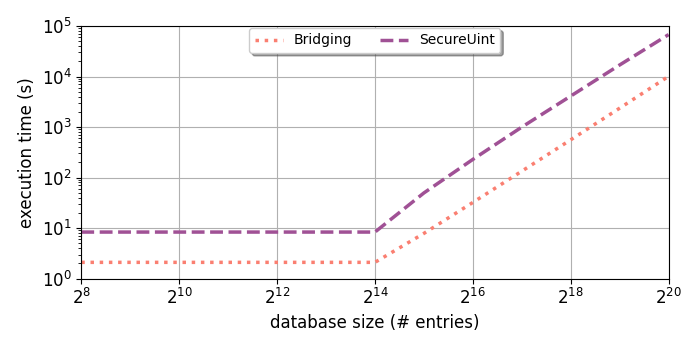
\includegraphics[width=\linewidth]{img/application.png}}
	\caption{Execution time of the setup protocol of a URL denylisting application \cite{urldenylist} implementing the Private Membership Test.}
	\label{fig:application}
\end{figure}

This performance improvement is enabled with just a few tweaks to the sort algorithm.
Consider Listing \ref{list:pmt_sort} presenting this algorithm as an example of modifications required to enable bridged computation.
Function \texttt{sort} reorders the items of a Bloom filter in a sequence known only to the client using encrypted variable \texttt{order}. It creates a list of plaintext indices according to the protocol (lines 10-23), compares homomorphically with the encrypted list of unique permutations sent by the client (variable \texttt{order}), and composes the encrypted Bloom filter \texttt{efilter} with values in this particular order (lines 25-42).

The homomorphic operations start after line 24. There are only a few necessary changes to the algorithm: 1) In lines 1, 26, and 31 we change the return and variable types from \texttt{vector<\secuint<S>{}>} to \texttt{vector<\secmod>}, and 2) in line 35, we cast the \secbool\ type to \secmod, so the subsequent multiplication is done using modular arithmetic.
In bit-level arithmetic it is faster to cast the \texttt{vector<int>} to \secuint\ and multiply by a \secbool, since it results in a \secbool-\secuint\ multiplication instead of a \secuint-\texttt{vector<int>} multiplication. Nevertheless, with bridging it is faster to cast the \secbool\ to \secmod, instead of \texttt{vector<int>}, because \secmod-\texttt{vector<int>} multiplication is faster and less noisy than \secmod-\secmod\ multiplication.
As can be seen in Fig. \ref{fig:application}, Bridging unlocks {\it one order of magnitude} performance improvement, and it only requires minor changes to the source code.
